\begin{enumerate}
\item \begin{enumerate}
\item D'après sa dérivée
\begin{displaymath}
 f'_{n}(t)=\frac{1}{n!}(n-t)t^{n-1}e^{-t}
\end{displaymath}
la fonction $f_{n}$ est croissante de 0 à $n$, décroissante ensuite.
Elle atteint sa borne supérieure en $n$:
\begin{displaymath}
M_{n}=f_{n}(n)=\frac{n^{n}e^{-n}}{n!}.
\end{displaymath}

\item On forme le quotient de deux termes consécutifs
\begin{multline*}
\frac{M_{n+1}}{M_{n}}
  = \frac{(n+1)^{n+1}e^{-(n+1)}}{(n+1)!}\frac{n!}{n^{n}e^{-n}} \\
  = \left(\frac{n+1}{n}\right)^{n}e^{-1}
  = \left(1+\frac{1}{n}\right)^{n}e^{-1}=e^{-1+n\ln (1+\frac{1}{n})}.
\end{multline*}
Comme $\ln (1+x)\leq x$ pour $x\geq 0$ (concavité de $\ln$); pour $x=\frac{1}{n}$,
\begin{displaymath}
 -1+n\ln (1+\frac{1}{n})\leq 0\; \text{ et } \; \frac{M_{n+1}}{M_{n}}\leq 1.
\end{displaymath}

\item La suite $(M_n)$ est décroissante donc elle est bornée par son premier terme.
\begin{displaymath}
   M = M_{1} = \frac{1}{n}.
\end{displaymath}
Le calcul de $\int_{0}^{+\infty}\frac{t^{n}e^{-t}}{n!}\,dt$ se fait par récurrence à l'aide d'une intégration par parties. On trouve
\begin{displaymath}
  \int_{0}^{+\infty}\frac{t^{n}e^{-t}}{n!}\,dt = 1.
\end{displaymath}

\item Cas $a_{n}=(-1)^{n}$.
\begin{displaymath}
  \left(\sum _{k=0}^{n}\frac{(-t)^{k}}{k!}\right)_{n\in \mathbb{N}}\rightarrow e^{-t}  \Rightarrow
  \left(\sum _{k=0}^{n}\frac{(-1)^{k}t^{k}e^{-t}}{k!}\right)_{n\in \mathbb{N}}\rightarrow e^{-2t}.
\end{displaymath}
qui est intégrable.

Cas $a_{n}=(-1)^{n}n$. La somme démarre alors en $k=1$ et on peut décaler les indices
\begin{displaymath}
  \sum _{k=0}^{n}\frac{(-1)^{k} k t^{k}e^{-t}}{k!}= (-t)\sum _{k=1}^{n-1}\frac{(-1)^{k-1}t^{k-1}e^{-t}}{(k-1)!}.
\end{displaymath}
Cette suite converge vers $-te^{-2t}$ qui est intégrable. Les deux séries alternées considérées convergent donc au sens de $(f_{n})$.
\end{enumerate}
\item \begin{enumerate}
\item Les fonctions sont affines par morceaux. Chaque graphe est formé d'un triangle de base 2 et de hauteur 1. Pour les fonctions $f_0$, $f_1$, $f_2$, $f_3$, les abcisses des sommets sont respectivement $1$, $2$, $3$, $4$.
\begin{figure}
   \centering
   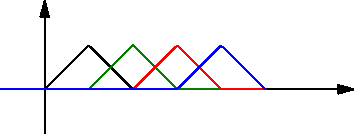
\includegraphics{Cbertr_1.pdf}
   \caption{2.a. Représentations graphiques de $f_0$, $f_1$, $f_2$, $f_3$.}
\end{figure}
\item La famille est de Bertrand car les bornes supérieures et les intégrales valent 1 (aire du triangle).
\item Pour tout $t$ fixé, la suite $(a_n f_{n}(t))_{n\in \mathbb{N}}$ est nulle à partir d'un certain rang. La suite $(\sum _{k=0}^{n}a_k f_{k}(t))_{n\in \mathbb{N}}$ est stationnaire donc convergente.

Si $t\in [p,p+1]$, seules $f_{p}(t)$ et $f_{p+1}(t)$ ne sont pas nulles parmi les $f_{k}(t)$, donc $f(t)=a_{p}f_{p}(t)+ a_{p+1}f_{p+1}(t)$ et
$$\int_{p}^{p+1}f(t)\,dt=\frac{a_{p}+a_{p+1}}{2}$$
\item Si $(\sum _{k=0}^{n}a_{k})_{n\in \mathbb{N}}$ converge, il en est de même de $(\sum _{k=0}^{n} \frac{ a_{k}+ a_{k+1}}{2})_{n\in \mathbb{N}}$ donc la série converge au sens de $(f_{n})$

On a vu en 1.d. que $\sum (-1)^{n}$ convergeait au sens de $(\frac{t^{n}e^{-t}}{n!})$ mais divergeait au sens usuel.
\end{enumerate}
\end{enumerate}
